\documentclass[11pt,letterpaper]{article}
\usepackage{times}
\usepackage[onehalfspacing]{setspace}
\usepackage{natbib}\bibpunct{(}{)}{,}{}{}{,}
\usepackage{amsmath,amsfonts,amsthm}
\usepackage{comment}
\usepackage{tabularx}
\usepackage{multirow}
\usepackage{booktabs}
\usepackage{subcaption}
\usepackage{graphicx}
\usepackage[colorlinks,linkcolor=blue,citecolor=black,urlcolor=black]{hyperref}
\usepackage[title,titletoc]{appendix}
\usepackage{enumitem}
\usepackage{subcaption}  % For subfigures
\usepackage{lscape}      % For landscape orientation if needed
\usepackage[noabbrev,capitalize]{cleveref}
\usepackage{tikz}
\usetikzlibrary{shapes.geometric}
\usepackage{pgfplots}
\usetikzlibrary{patterns, pgfplots.fillbetween}
\usepackage{graphicx}
\usepackage{mathpazo}

% commands
\newtheorem{definition}{Definition}
\newtheorem{proposition}{Proposition}
\newtheorem{lemma}{Lemma}
\newcommand{\figpath}{fig/}
\newcommand{\tablepath}{table/}
\newcommand{\rmdi}{\mathrm{d}}

% table and figure formatting
%\input{formats}

% page size
\setlength{\textwidth}{\paperwidth}
\addtolength{\textwidth}{-1.7in}
\setlength{\oddsidemargin}{.85in}
\addtolength{\oddsidemargin}{-.85in}
\setlength{\evensidemargin}{\oddsidemargin}
\setlength{\headheight}{0pt}
\setlength{\headsep}{0pt}
\setlength{\textheight}{\paperheight}
\addtolength{\textheight}{-\headheight}
\addtolength{\textheight}{-\headsep}
\addtolength{\textheight}{-\footskip}
\addtolength{\textheight}{-1.75in}
\setlength{\topmargin}{1in}
\addtolength{\topmargin}{-1in}

\begin{document}

\title{\textbf{Classical Ricardian Trade: Two Countries, Two Goods}}
\author{\large%
\setcounter{footnote}{0}%
Carlos G\'{o}es \\[-3pt] \textit{\small IFC, World Bank Group}
}
\maketitle

\paragraph{Production} The simplest Ricardian trade model goes back to... David Ricardo. Consider a world with 2 countries $i \in \{ US, COL\}$ and two products $p \in \{ C, R\}$. In country $i$, there are $L_i$ units of labor (worker-hours) available, which we call the labor endowment. An inherent technological characteristic of country $i$ are \textbf{unit labor requirements}, i.e. to produce one unit of good $p$ firms in country $i$ use $a_{i,p}$ units of labor. In country $i$, firms producing good $p$ maximize profits under perfect competition:
        \begin{equation}\label{eq: production}
            \max_{Y_{i,p}} \pi_{i,p} = \max_{Y_{i,p}} P_{i,p}Y_{i,p} - w_i a_{i,p} Y_{i,p} 
        \end{equation}

Labor is mobile. This means that labor can be distributed for the production of either good, such that and the same pool of workers can be allocated to either good. For that reason, total labor endowment must respect the following constraint:

\begin{equation}\label{eq: ppf-inequality}
    \underbrace{a_{i,C} \times Y_{i,C}}_{\substack{\text{labor used in} \\ \text{production of } C}} + \underbrace{a_{i,R} \times Y_{i,R}}_{\substack{\text{labor used in} \\ \text{production of } R}} \le \underbrace{L_i}_{\substack{\text{total labor} \\ \text{available in } i}}
\end{equation}

The inequality above defines set of feasible production choices. This set define potential choices of $(Y_{i,C}, Y_{i,R})$ that are ``feasible.'' That is, if the labor input used to produce $(Y_{i,C}, Y_{i,R})$ is not larger than $L_i$, production is feasible:

        \begin{equation*}
            \mathcal{Y}_{i} := \{ (Y_{i,C}, Y_{i,R}) : a_{i,C} \times Y_{i,C} + a_{i,R} \times Y_{i,R} \le L_i \}
        \end{equation*}


\begin{figure}[htbp!]
\centering
\begin{tikzpicture}
\begin{axis}[
    xlabel={Quantity of roses, $Y_{i,R}$},
    ylabel={Quantity of computers, $Y_{i,C}$},
    xmin=0, xmax=11,
    ymin=0, ymax=0.11,
    yticklabel=\empty,
    xticklabel=\empty,
    axis lines=left,
    enlargelimits=false,
    clip=false,
    axis on top,
    scaled x ticks=false,
    width=9cm, height=7cm,
    title style={font=\bfseries}
]

% Filled triangle under the PPF
\addplot [
    name path=A,
    domain=0:0.1,
    draw=none
] {.1 - 1/100*x};

\path[name path=B] (axis cs:0,0) -- (axis cs:10,0);

\addplot [
    fill=cyan!20,
    draw=none
] fill between [of=A and B];

% PPF line
\addplot[thick, blue, domain=0:10] {.1 - 1/100*x};

% Labels
\node at (axis cs:3.5,0.03) {\Large $\mathcal{Y}_{i}$};
\node at (axis cs:10,-.01) {\scriptsize $\frac{L_{i}}{a_{i,R}}$};
\node at (axis cs:-.75,.1) {\scriptsize $\frac{L_{i}}{a_{i,C}}$};
\node at (axis cs:10,0.05) { $\textcolor{blue}{Y_{i,C} = \frac{L_{i}}{a_{i,C}} - \frac{a_{i,R}}{a_{i,C}} \times Y_{i,R}}$};

\end{axis}
\end{tikzpicture}
\caption{Set of feasible production $\mathcal{Y}_i$ and the Production Possibilities Frontier}\label{fig: pp-sets}
\end{figure}
            
A graphical representation of $\mathcal{Y}_i$ is in Figure \ref{fig: pp-sets}. Every choice of $(Y_{i,C}, Y_{i,R})$ in the cyan triangle is feasible. In English, being feasible means that there is enough labor in $i$ to produce the combination of output that falls within the triangle. If the choices $(Y_{i,C}, Y_{i,R})$ fall \textit{on the blue line} (the boundary of set), then \textit{total production exhausts available labor}. This means that the weak inequality in \eqref{eq: ppf-inequality} holds equality. In other words, the blue line is defined by the equation $a_{i,C} \times Y_{i,C} + a_{i,R} \times Y_{i,R} = L_i$, which can be rearranged to solved for $Y_{i,C}$ as $Y_{i,C} = \frac{L_{i}}{a_{i,C}} - \frac{a_{i,R}}{a_{i,C}} \times Y_{i,R}$. We call the blue line the \textbf{production possibilities frontier} (PPF).

Since labor only one type of labor (mobile across sectors), there is a single wage $w_i$. In equilibrium, if production for good $p$ happens, \textbf{prices equal marginal cost} (take the derivative of \eqref{eq: production} above with respect to $Y_{i,p}$):

        \begin{eqnarray*}
            P_{i,p} = w_i a_{i,p} \iff \frac{P_{i,p}}{a_{i,p}} = w_i  \qquad \text{ for } p \in\{C,R\}
        \end{eqnarray*}

\paragraph{Demand} Workers in each country $i$ inelastically supply their labor and earn labor income $w_i L_i$. They have preferences over goods $p \in \{ C, R\}$. They purchase quantities $Q_{i,C}, Q_{i,R}$ for prices $P_{i,C}, P_{i,R}$ and exhaust their labor income, maximizing:

\begin{equation*}
    \max_{\{Q_{i,C}, Q_{i,R}\}} U_i(Q_{i,C}, Q_{i,R}) \equiv Q_{i,C}^{\alpha_i} Q_{i,R}^{1-\alpha_i} \qquad s.t. \qquad P_{i,C} Q_{i,C} + P_{i,R} Q_{i,R} = w_i L_i
\end{equation*}

This is a simple constrained concave maximization problem, that you should know how to solve from your calculus classes. One way to solve it is to replace the constraint into the objective function. Note $Q_{i,R} = \frac{w_i L_i}{P_{i,R}} - \frac{P_{i,C}}{P_{i,R} } Q_{i,C}$, so the maximization problem below is equivalent to the original one:

\begin{equation*}
    \max_{\{Q_{i,C}\}} U_i(Q_{i,C}, Q_{i,R}(Q_{i,C})) \equiv Q_{i,C}^{\alpha_i} \left( \frac{w_i L_i}{P_{i,R}} - \frac{P_{i,C}}{P_{i,R} } Q_{i,C} \right)^{1-\alpha_i}
\end{equation*}

\noindent for which we can take a derivative and set it equal to zero to find the optimal point:

\scriptsize{
\begin{eqnarray*}
    & & \alpha_i Q_{i,C}^{\alpha_i-1} \left( \underbrace{\frac{w_i L_i}{P_{i,R}} - \frac{P_{i,C}}{P_{i,R} } Q_{i,C}}_{=Q_{i,R}} \right)^{1-\alpha_i} + Q_{i,C}^{\alpha_i} (1-\alpha_i) \left( \underbrace{\frac{w_i L_i}{P_{i,R}} - \frac{P_{i,C}}{P_{i,R} } Q_{i,C}}_{=Q_{i,R}} \right)^{1-\alpha_i-1} \left( - \frac{P_{i,C}}{P_{i,R}}\right) = 0 \\
%    & & \alpha_i  \left( \frac{Q_{i,R}}{Q_{i,C}} \right)^{1-\alpha_i} - (1-\alpha_i) \left( \frac{Q_{i,R}}{Q_{i,C}} \right)^{-\alpha_i} \left( \frac{P_{i,C}}{P_{i,R}}\right) = 0 \\
%    & & \alpha_i  \left( \frac{Q_{i,R}}{Q_{i,C}} \right)^{1-\alpha_i} = (1-\alpha_i) \left( \frac{Q_{i,R}}{Q_{i,C}} \right)^{-\alpha_i} \left( \frac{P_{i,C}}{P_{i,R}}\right) \\
%    & & \frac{Q_{i,R}}{Q_{i,C}}  = \frac{1-\alpha_i}{\alpha_i } \left( \frac{P_{i,C}}{P_{i,R}}\right) \\
\iff    & & Q_{i,R}  = \frac{1-\alpha_i}{\alpha_i } \left( \frac{P_{i,C}}{P_{i,R}}\right) Q_{i,C}
\end{eqnarray*}
}

\normalsize
Replacing the last line into the budget constraint:

\scriptsize{
\begin{eqnarray*}
    Q_{i,R}&=& \frac{w_i L_i}{P_{i,R}} - \frac{P_{i,C}}{P_{i,R} } Q_{i,C} \\
    \frac{1-\alpha_i}{\alpha_i } \left( \frac{P_{i,C}}{P_{i,R}}\right) Q_{i,C} &=& \frac{w_i L_i}{P_{i,R}} - \frac{P_{i,C}}{P_{i,R} } Q_{i,C} \\
%    \frac{1-\alpha_i}{\alpha_i } \left( \frac{P_{i,C}}{P_{i,R}}\right) Q_{i,C} + \frac{P_{i,C}}{P_{i,R} } Q_{i,C} &=& \frac{w_i L_i}{P_{i,R}}  \\
%    \frac{1-\alpha_i + \alpha_i}{\alpha_i } \left( \frac{P_{i,C}}{P_{i,R}}\right) Q_{i,C} &=& \frac{w_i L_i}{P_{i,R}}  \\
    Q_{i,C} &=& \alpha_i  \frac{w_i L_i}{P_{i,C}}
\end{eqnarray*}

}

\normalsize
Finally:
{\scriptsize
\begin{eqnarray*}
     Q_{i,R}  &=& \frac{1-\alpha_i}{\alpha_i } \left( \frac{P_{i,C}}{P_{i,R}}\right) Q_{i,C}  \\
     Q_{i,R}  &=& \frac{1-\alpha_i}{\alpha_i } \left( \frac{P_{i,C}}{P_{i,R}}\right) \alpha_i  \frac{w_i L_i}{P_{i,C}} \\
      Q_{i,R}  &=& (1-\alpha_i) \frac{w_i L_i}{P_{i,R}}
\end{eqnarray*}
}
\normalsize
Therefore, optimal demand functions satisfy:

\begin{equation}\label{eq: demand}
    Q_{i,C} = \alpha_i  \frac{w_i L_i}{P_{i,C}}, \qquad Q_{i,R} = (1-\alpha_i) \frac{w_i L_i}{P_{i,R}}
\end{equation}
\normalsize

Under Cobb-Douglas preferences, each consumer allocates a fixed share of their income—determined by their preference parameter $(\alpha_i, 1-\alpha_i)$ to each good, purchasing quantities inversely proportional to the price of that good. This holds regardless of whether consumers are in autarky or trade. 

\paragraph{Autarky prices and equilibrium} In autarky, since there is demand for both goods, there there will be production in both sectors. Therefore, \textbf{in the autarky equilibrium}, we can pin down the relative wage $P_{i,C} / P_{i,R}$:

\begin{equation}\label{eq: autarky-prices}
            \frac{P_{i,C}}{a_{i,C}} = w_i = \frac{P_{i,R}}{a_{i,R}} \iff \frac{P_{i,C}}{P_{i,R}} = \frac{a_{i,C}}{a_{i,R}}  
\end{equation}

Hence, in autarky, relative prices will reflect the \textbf{opportunity cost} within country $i$. Replacing for wages in \eqref{eq: demand}, we can solve for optimal demanded quantities in autarky as a function of parameters:

\begin{equation}\label{eq: demand-autarky}
    Q_{i,C} = \alpha_i  \frac{w_i L_i}{P_{i,C}} = \alpha_i  \frac{L_i}{a_{i,C}}  , \qquad Q_{i,R} = (1-\alpha_i) \frac{w_i L_i}{P_{i,R}} = (1-\alpha_i) \frac{L_i}{a_{i,R}} 
\end{equation}

Finally, in equilibrium, it must be the case that \textbf{supply equals demand}. We call that the \textbf{market clearing condition}. In the autarky equilibrium, this is simply stating that $Y_{i,C} = Q_{i,C}$ and $Y_{i,R} = Q_{i,R}$. Since we have solved for optimal demands $( Q_{i,C}, Q_{i,R})$ using the market clearing condition gives us the optimal supply $(Y_{i,C}, Y_{i,R})$. To make sure that production is feasible and this is an equilibrium, we can check that these choices satisfy the PPF:
\begin{eqnarray*}
    a_{i,C} \times Y_{i,C} + a_{i,R} \times Y_{i,R} &=& L_i \\
    a_{i,C} \times Q_{i,C} + a_{i,R} \times Q_{i,R} &=& L_i \qquad (\text{mkt clearing}) \\
    a_{i,C} \times \alpha_i  \frac{L_i}{a_{i,C}} + a_{i,R} \times (1-\alpha_i) \frac{L_i}{a_{i,R}}  &=& L_i \qquad (\text{optimal demand}) \\
    \alpha_i  L_i + (1-\alpha_i) L_i  &=& L_i \qquad (\text{checks out!})
\end{eqnarray*}

Given the solutions above, and a set of parameters $(L_i, \alpha_i, a_{i,C}, a_{i,R})_{i \in \{COL, US\}}$, we can immediately solve for the numerical solutions in an autarky equilibrium. An example is in Table \ref{tab: autarky-num}. With those values at hand, it is easy to plot the autarky equilibrium in two charts, as we do in Figure \ref{fig: autarky-num}.

\begin{table}[htbp]
\centering
\begin{tabular}{lcc}
\toprule
\textbf{Variable} & \textbf{United States (US)} & \textbf{Colombia (COL)} \\
\midrule
Labor endowment $L_i$ & 300 million & 54 million \\
Preference parameters $\alpha_i$ & 1/2 & 3/4 \\
Unit labor requirement for computers $a_{i,C}$ & 3{,}000 & 5{,}400 \\
Unit labor requirement for roses $a_{i,R}$ & 30 & 6 \\
\midrule
Maximum computers: $\frac{L_{i}}{a_{i,C}}$ & $\frac{300 \text{m}}{3{,}000} = 100{,}000$ & $\frac{54 \text{m}}{5{,}400} = 10{,}000$ \\
Maximum roses: $\frac{L_{i}}{a_{i,R}}$ & $\frac{300 \text{m}}{30} = 10 \text{m}$ & $\frac{54 \text{m}}{6} = 9 \text{m}$ \\
\midrule
Relative Prices (-slope of PPF): $\frac{P_{i,C}}{a_{i,R}} = \frac{a_{i,C}}{a_{i,R}}$ & $\frac{3{,}000}{30} = 100$ & $\frac{5{,}400}{6} = 900$ \\
Demand and supply of computers: $\alpha_i  \frac{L_i}{a_{i,C}}$ & $1/2 \times \frac{300 \text{m}}{3{,}000} = 50{,}000$ & $3/4 \times \frac{54 \text{m}}{5{,}400} = 7{,}500$ \\
Demand and supply of roses: $(1-\alpha_i)  \frac{L_i}{a_{i,R}}$ & $1/2 \times \frac{300 \text{m}}{30} = 5 \text{m}$ & $3/4 \times \frac{54 \text{m}}{6} = 2{.}25 \text{m}$ \\
\bottomrule
\end{tabular}
\caption{Labor, unit requirements, and opportunity costs}\label{tab: autarky-num}
\end{table}


\begin{figure}[htbp!]

% California
\begin{subfigure}{0.5\linewidth}
\resizebox{\linewidth}{!}{%
\begin{tikzpicture}
\pgfmathsetmacro{\aC}{100}       % unit labor requirement for computers
\pgfmathsetmacro{\aR}{1}         % unit labor requirement for roses
\pgfmathsetmacro{\alpha}{0.5}    % preference for computers
\pgfmathsetmacro{\Lendow}{10}    % labor endowment

% Compute equilibrium quantities
\pgfmathsetmacro{\Qc}{(\alpha*\Lendow)/\aC}
\pgfmathsetmacro{\Qr}{((1 - \alpha)*\Lendow)/\aR}

% Compute utility level
\pgfmathsetmacro{\U}{(\Qc^(\alpha))*(\Qr^(1 - \alpha))}

% Compute prefactor for indifference curve: Qc = A * Qr^(- (1 - alpha)/alpha)
\pgfmathsetmacro{\expo}{(1 - \alpha)/\alpha}
\pgfmathsetmacro{\A}{\U^(1/\alpha)}

\centering
\begin{axis}[
    ylabel={Quantity of computers, $\textcolor{red}{Q_{US,C}}, \textcolor{blue}{Y_{US,C}}$},
    xlabel={Quantity of roses, $\textcolor{red}{Q_{US,R}}, \textcolor{blue}{Y_{US,R}}$},
    ymin=0, ymax=0.11,
    xmin=0, xmax=11,
    yticklabel=\empty,
    xticklabel=\empty,
    axis lines=left,
    enlargelimits=false,
    clip=false,
    axis on top,
    scaled x ticks=false,
    width=9cm, height=7cm,
    title style={font=\bfseries}
]

% PPF: Q_C = (L/a_C) - (a_R/a_C) * Q_R
\addplot[thick, blue, domain=0:10] {\Lendow/\aC - (\aR/\aC)*x};

% Indifference curve through optimal bundle
\addplot[thick, brown, domain=2.5:10, samples=100] {\A * x^(-\expo)};

% Labels
%\node at (axis cs:3.5,0.03) {\Large $\mathcal{Y}_{US}$};
\node at (axis cs:\Lendow/\aR,-.01) {\scriptsize $\frac{L_{US}}{a_{US,R}}$};
\node at (axis cs:-.75,\Lendow/\aC) {\scriptsize $\frac{L_{US}}{a_{US,C}}$};


% Equilibrium point
\addplot[only marks, mark=*, color=blue, mark size=2pt] coordinates {(\Qr, \Qc)};
\node at (axis cs:\Qr - 1.25,\Qc - 0.005) {\scriptsize $\textcolor{blue}{(Q_{US,R},Q_{US,C})}$};
\node at (axis cs:\Qr - 2,\Qc + 0.0025) {\scriptsize $\textcolor{blue}{(Y_{US,R},Y_{US,C})}$};



\end{axis}

\end{tikzpicture}
}
\end{subfigure}
%
% Colombia
\begin{subfigure}{0.5\textwidth}
\resizebox{\linewidth}{!}{%

\begin{tikzpicture}
\pgfmathsetmacro{\aC}{900}       % unit labor requirement for computers
\pgfmathsetmacro{\aR}{1}         % unit labor requirement for roses
\pgfmathsetmacro{\alpha}{0.75}    % preference for computers
\pgfmathsetmacro{\Lendow}{9}    % labor endowment

% Compute equilibrium quantities
\pgfmathsetmacro{\Qc}{(\alpha*\Lendow)/\aC}
\pgfmathsetmacro{\Qr}{((1 - \alpha)*\Lendow)/\aR}

% Compute utility level
\pgfmathsetmacro{\U}{(\Qc^(\alpha))*(\Qr^(1 - \alpha))}

% Compute prefactor for indifference curve: Qc = A * Qr^(- (1 - alpha)/alpha)
\pgfmathsetmacro{\expo}{(1 - \alpha)/\alpha}
\pgfmathsetmacro{\A}{\U^(1/\alpha)}

\centering
\begin{axis}[
    ylabel={Quantity of computers, $\textcolor{red}{Q_{COL,C}}, \textcolor{blue}{Y_{COL,C}}$},
    xlabel={Quantity of roses, $\textcolor{red}{Q_{COL,R}}, \textcolor{blue}{Y_{COL,R}}$},
    ymin=0, ymax=0.11,
    xmin=0, xmax=11,
    yticklabel=\empty,
    xticklabel=\empty,
    axis lines=left,
    enlargelimits=false,
    clip=false,
    axis on top,
    scaled x ticks=false,
    width=9cm, height=7cm,
    title style={font=\bfseries}
]

% PPF: Q_C = (L/a_C) - (a_R/a_C) * Q_R
\addplot[thick, blue, domain=0:9] {\Lendow/\aC - (\aR/\aC)*x};

% Indifference curve through optimal bundle
\addplot[brown, domain=0.1:9, samples=100] {\A * x^(-\expo)};

% Labels

%\node at (axis cs:3.5,0.03) {\Large $\mathcal{Y}_{US}$};
\node at (axis cs:\Lendow/\aR,-.01) {\scriptsize $\frac{L_{COL}}{a_{COL,R}}$};
\node at (axis cs:-.75,\Lendow/\aC) {\scriptsize $\frac{L_{COL}}{a_{COL,C}}$};


% Equilibrium point
\addplot[only marks, mark=*, color=blue, mark size=2pt] coordinates {(\Qr, \Qc)};
\node at (axis cs:\Qr + 1.25,\Qc + 0.009) {\scriptsize $\textcolor{blue}{(Q_{COL,R},Q_{COL,C})}$};
\node at (axis cs:\Qr + 2.25,\Qc + 0.001) {\scriptsize $\textcolor{blue}{(Y_{COL,R},Y_{COL,C})}$};


\end{axis}

\end{tikzpicture}
}

\end{subfigure}

\caption{Autarky equilibrium}\label{fig: autarky-num}

\end{figure}

\newpage


\paragraph{Free trade prices and equilibrium} We say Colombia has an \textbf{absolute advantage} in the production of good $p$ if $a_{COL,p} < a_{US,p}$. In other words, having an  absolute advantage in production means that a country is more productive: it uses less labor to produce one unit. 

Recall that, to respect the PPF, in order to produce more of one good, it needs to give up production of the other good. Since a country forgoes roses to produce computers, the \textbf{opportunity cost} of computers can be measured in terms of roses. We say a country has a \textbf{comparative advantage} in producing a good if its opportunity cost of the good is lower than in the rest of the world.

For instance, we say Colombia has an \textbf{comparative advantage} in the production of roses, since: $1/900 = a_{COL,R}/a_{COL,C} < a_{US,R}/a_{US,C} = 1/100$. Similarly, we say the US has an \textbf{comparative advantage} in the production of computers, since: $900 = a_{COL,C}/a_{COL,R} > a_{US,C}/a_{US,R} = 100$.

First, note that under free trade there will be world prices for each good $P_C, P_R$ that will be the \textit{same across countries}. Second, we know from the autarky equilibrium, if the relative price is exactly equal to the marginal cost of shift production $\frac{P_{i,C}}{P_{i,R}} = \frac{a_{i,C}}{a_{i,R}}$, then a country can supply any of the products and workers would be indifferent between producing computers or roses (their wage would be the same in either sector).

But suppose that, under the world equilibrium, $\frac{P_{C}}{P_{R}} > \frac{a_{i,C}}{a_{i,R}}$. What would happen? This inequality states that the relative marginal revenue of computers in country $i$ is \textit{greater than its relative marginal cost}. As a consequence, country $i$ would shift all of its workers to the production of computers. Likewise, if $\frac{P_{C}}{P_{R}} < \frac{a_{i,C}}{a_{i,R}}$ the relative marginal revenue of computers in country $i$ is \textit{smaller than its relative marginal cost}. As a consequence, country $i$ would shift all of its workers to the production of roses. 

Consider once again the numerical examples in Table \ref{tab: autarky-num}. Suppose that $P_C/P_R = a_{US,C}/ a_{US,R}$. In that case, prices would be the same in the US as in autarky, so the production of computers in the US $Y_{US,C}$ could range anywhere from zero to 100,000 (with production of roses $Y_{US,R}$ ranging from 10 million to zero). However, since $a_{US,C}/ a_{US,R} < a_{COL,C}/a_{COL,R}$, this implies that $P_C/P_R < a_{COL,C}/a_{COL,R}$. So Colombia would fully specialize in the production of roses ($Y_{COL,R} = L_{COL}/a_{COL,R}$ and $Y_{COL,C} = 0$).

Conversely, suppose that that $P_C/P_R = a_{COL,C}/ a_{COL,R}$. In that case, Colombia would be indifferent between producing computers and roses and its production of computers $Y_{COL,C}$ could range anywhere from zero to 10,000 (with production of roses $Y_{COL,R}$ ranging from 9 million to zero). However, since $a_{US,C}/ a_{US,R} < a_{COL,C}/a_{COL,R}$, this implies that $P_C/P_R > a_{US,C}/ a_{US,R}$. So the US would fully specialize in the production of computers ($Y_{US,C} = L_{US}/a_{US,C}$ and $Y_{US,R} = 0$).

Each country specializes in the good in which they have a comparative advantage if the relative price $P_C/P_R$ is such that:

\begin{equation}\label{eq: price-trade}
    \frac{a_{US,C}}{a_{US,R}} < \frac{P_C}{P_R} < \frac{a_{COL,C}}{a_{COL,R}}
\end{equation}

In the bottom segment of Figure \ref{fig: relative-supply}, production of computers in the US ranges from 0 to 100,000 while Colombia is fully specialized in roses. In the top segment of the same figure, production of computers in Colombia ranges from 0 to 10,000 while the US is fully specialized in computers. In the vertical segment, relative prices satisfy equation  \eqref{eq: price-trade}, so both countries are fully specialized. In that case, the global supply of computers is $L_{US}/a_{US,C} = 100{,}000$ and the global supply of roses is $L_{COL}/a_{COL,R} = 9{,}000{,}000$.


\begin{figure}[htpd!]
\centering
\begin{tikzpicture}
\begin{axis}[
    ylabel={Relative price of computers $\frac{P_C}{P_R}$},
    xlabel={Relative quantity of computers $\textcolor{blue}{\frac{Y_{C}}{Y_{R}} = \frac{Y_{COL,C}+Y_{US,C}}{Y_{COL,R}+Y_{US,R}} }$},
    ymin=0, ymax=3,
    xmin=0, xmax=2,
    yticklabel=\empty,
    xticklabel=\empty,
    axis lines=left,
    enlargelimits=false,
    clip=false,
    axis on top,
    scaled x ticks=false,
    width=9cm, height=7cm,
    title style={font=\bfseries}]

% Relative Supply RS
\addplot[thick, blue] coordinates {(0,1) (0.8,1.0)};
\addplot[thick, blue] coordinates {(0.8,1.0) (0.8,2.0)};
\addplot[thick, blue] coordinates {(0.8,2.0) (1.6,2.0)};
%\node at (axis cs:1.65,2.7) {\small $RS$};

% Dashed lines for autarky prices
\addplot[dashed] coordinates {(0,2.0) (0.8,2.0)};
\node at (axis cs:-0.15,2) {$\frac{a_{COL,C}}{a_{COL,R}}$};

\addplot[dashed] coordinates {(0.8,1.0) (1.6,1.0)};
\node at (axis cs:-0.15,1) {$\frac{a_{US,C}}{a_{US,R}}$};


% Vertical dashed lines for quantities
\addplot[dashed] coordinates {(0.8,0) (0.8,1.0)};
\node at (axis cs:0.8,-0.2) {$\frac{L_{US}/a_{US,C}}{L_{COL}/a_{COL,R}}$};

\end{axis}
\end{tikzpicture}
\caption{Relative Supply of Computers as a function of Relative Prices}\label{fig: relative-supply}
\end{figure}

How are prices determined in a free trade equilibrium? Relative prices will adjust to make sure that the global supply for each good equals its global demand. First we need to determine the global supply of each good. But we have already done so: the US fully specializes in computers $Y^T_{C} = L_{US}/a_{US,C} = 100{,}000$ and Colombia fully specializes in roses  $Y^T_R = L_{COL}/a_{COL,R} = 9{,}000{,}000$. Global demand for computers and roses satisfy, respectively:

\begin{eqnarray*}
    Q_{C} &\equiv& Q^T_{US,C} +  Q^T_{COL,C} = \alpha_{US} \frac{w_{US} L_{US} }{P_C} + \alpha_{COL} \frac{w_{COL} L_{COL} }{P_C}  \\
    Q_{R} &\equiv& Q^T_{US,R} +  Q^T_{COL,R}  = (1-\alpha_{US}) \frac{w_{US} L_{US} }{P_R} + (1-\alpha_{COL}) \frac{w_{COL} L_{COL} }{P_R}    
\end{eqnarray*}

Note that the relative global demand for computers $Q_C/Q_R$ is decreasing in relative prices $P_C / P_R$ (if you are not convinced, write down the expression for $Q_C/Q_R$ and note that you can factor out $P_C / P_R$).  This is also expected. As the relative price of computers rises, consumers will tend to purchase less computers and more roses, so the relative demand for computers falls.

Graphically, we can draw a downward sloping global demand curve. In Figure  a trade equilibrium, if demand is such that it satisfies \eqref{eq: price-trade}, then both countries will specialize and 

\begin{figure}[htpd!]
\centering
\begin{tikzpicture}
\begin{axis}[
    ylabel={Relative price of computers $\frac{P_C}{P_R}$},
    xlabel={Relative quantity of computers $\textcolor{red}{\frac{Q_{C}}{Q_{R}} } , \textcolor{blue}{\frac{Y_{C}}{Y_{R}} }$},
    ymin=0, ymax=3,
    xmin=0, xmax=2,
    yticklabel=\empty,
    xticklabel=\empty,
    axis lines=left,
    enlargelimits=false,
    clip=false,
    axis on top,
    scaled x ticks=false,
    width=9cm, height=7cm,
    title style={font=\bfseries}]

% Relative Demand RD
\addplot[
    red, thick,
    domain=0.45:1.8,
    samples=100
] {1.2/(x)};
%\node[red] at (axis cs:1.4,1.25) {\small $RD$};

% Relative Supply RS
\addplot[thick, blue] coordinates {(0,1) (0.8,1.0)};
\addplot[thick, blue] coordinates {(0.8,1.0) (0.8,2.0)};
\addplot[thick, blue] coordinates {(0.8,2.0) (1.6,2.0)};
%\node at (axis cs:1.65,2.7) {\small $RS$};

% Dashed lines for autarky prices
\addplot[dashed] coordinates {(0,2.0) (0.8,2.0)};
\node at (axis cs:-0.15,2) {$\frac{a_{COL,C}}{a_{COL,R}}$};

\addplot[dashed] coordinates {(0.8,1.0) (1.6,1.0)};
\node at (axis cs:-0.15,1) {$\frac{a_{US,C}}{a_{US,R}}$};

\addplot[dashed, red] coordinates {(0,1.5) (0.8,1.5)};

% Vertical dashed lines for quantities
\addplot[dashed] coordinates {(0.8,0) (0.8,1.0)};
\node at (axis cs:0.8,-0.2) {$\frac{L_{US}/a_{US,C}}{L_{COL}/a_{COL,R}}$};

\end{axis}
\end{tikzpicture}
\caption{Relative Supply and Demand of Computers as a Function of Relative Prices}
\end{figure}

\newpage


We have almost solved for the relative price. What is $w_{US}$, $w_{COL}$? Since there is only one sector operating in each country, we know that wages will be equal to the marginal product of each worker in the sector they are working, so $w_{US} = P_{C} / a_{US,C}$ and $w_{COL} = P_{R} / a_{COL,R}$. Therefore:
\begin{eqnarray*}
    Q_{C} = \alpha_{US} \frac{L_{US} }{a_{US,C}} + \alpha_{COL} \frac{L_{COL} }{a_{COL,R} \times  P_C/P_R}, Q_{R} = (1-\alpha_{US}) \times \frac{P_C}{P_R} \times \frac{ L_{US} }{a_{US,C}} + (1-\alpha_{COL}) \frac{L_{COL} }{a_{COL,R}}    
\end{eqnarray*}

We know have everything in terms of parameters, except for the relative price $P_C/P_R$. By setting global supply of either good equal to global demand, we can pin down those prices.  

\begin{eqnarray*}
    Q_{R} = (1-\alpha_{US}) \times \frac{P_C}{P_R} \times \frac{ L_{US} }{a_{US,C}} + (1-\alpha_{COL}) \frac{L_{COL} }{a_{COL,R}} &=& \frac{L_{COL} }{a_{COL,R}} = Y_R \\ 
\iff (1-\alpha_{US}) \times \frac{P_C}{P_R} \times \frac{ L_{US} }{a_{US,C}} &=& \alpha_{COL} \frac{L_{COL} }{a_{COL,R}} \\
\iff \frac{P_C}{P_R}  = \frac{\alpha_{COL}}{1-\alpha_{US}} \times \frac{L_{COL}/a_{COL,R}}{L_{US} / a_{US,C}} &=& \frac{3/4}{1/2} \times \frac{9 \text{m}}{100{,}000} \\ 
\iff \frac{P_C}{P_R} &=& 135
\end{eqnarray*}

With this at hand, we can calculate the demand for each product:

\begin{eqnarray*}
    Q^T_{US,C} &=& \alpha_{US} \frac{L_{US} }{a_{US,C}} = 1/2 \times \frac{300 \text{m}}{100{,}000} = 50,000 \\
    Q^T_{COL,C} &=& \alpha_{COL} \frac{L_{COL} }{a_{COL,R} \times P_C/P_R} = 3/4 \times \frac{54 \text{m}}{6 \times 135} = 50,000 \\
    Q^T_{US,R} &=& (1- \alpha_{US}) \times \frac{P_C}{P_R} \times \frac{L_{US} }{a_{US,C}} = 1/2 \times 135 \times \frac{300 \text{m}}{100{,}000} = 6,750,000 \\
    \qquad Q^T_{COL,R} &=& (1-\alpha_{COL}) \frac{L_{COL} }{a_{COL,R} } = 1/4 \times \frac{54 \text{m}}{6} = 2,250,000
\end{eqnarray*}

Expors of roses from Colombia to the US are $Y^T_{COL,R} - Q^T_{COL,R}$ while imports of computers from the US to Colombia are $Y^T_{US,C}-Q^T_{US,C}$. In equilibrium, since we are assuming balanced trade, \textbf{the value of exports must be equal to the value of imports}. We can check if that condition is satisfied and the market cleared with the values above:

\begin{eqnarray*}
    P_R \left( Y^T_{COL,R}- Q^T_{COL,R} \right) &=& P_C \left( Y^T_{US,C} - Q^T_{US,R} \right)  \\
    \left( 9{,}000{,}000 - 2{,}250{,}000 \right) &=& \frac{P_C}{P_R} \left( 100{,}000 - 50{,}000\right)  \\
      6{,}750{,}000  &=& 135 \times 50{,}000 \\
      6{,}750{,}000  &=& 6{,}750{,}000 \qquad \text{(checks out!)}
    \end{eqnarray*}

Finally, let us graph production ($Y$) and consumption ($Q$) both under \textcolor{blue}{autarky} and \textcolor{red}{free trade}, as done in Figure \ref{fig: trade-eq}. The slope of prices under autarky are equal to $-a_{i,R}/a_{i,C}$, equal to the slope of the PPF. Under free trade, the slope is the relative price $P_R/P_C = -1/135$. Note this is steeper than Colombia's PPF but flatter than the US' PPF (why?). Trade allows both countries to expand consumption and increase welfare (see higher indifference curves).

\begin{figure}[htbp]

% California
\begin{subfigure}{0.5\linewidth}
\resizebox{\linewidth}{!}{%
\begin{tikzpicture}
\pgfmathsetmacro{\aC}{100}       % unit labor requirement for computers
\pgfmathsetmacro{\aR}{1}         % unit labor requirement for roses
\pgfmathsetmacro{\alpha}{0.5}    % preference for computers
\pgfmathsetmacro{\Lendow}{10}    % labor endowment
\pgfmathsetmacro{\p}{135}    % trade price

% Compute equilibrium quantities
\pgfmathsetmacro{\Qc}{(\alpha*\Lendow)/\aC}
\pgfmathsetmacro{\Qr}{((1 - \alpha)*\Lendow)/\aR}
\pgfmathsetmacro{\QcT}{(\alpha*\Lendow)/\aC}
\pgfmathsetmacro{\QrT}{((1 - \alpha)*\p*\Lendow)/\aC}

% Compute utility level
\pgfmathsetmacro{\U}{(\Qc^(\alpha))*(\Qr^(1 - \alpha))}
\pgfmathsetmacro{\UT}{(\QcT^(\alpha))*(\QrT^(1 - \alpha))}

% Compute prefactor for indifference curve: Qc = A * Qr^(- (1 - alpha)/alpha)
\pgfmathsetmacro{\expo}{(1 - \alpha)/\alpha}
\pgfmathsetmacro{\A}{\U^(1/\alpha)}
\pgfmathsetmacro{\AT}{\UT^(1/\alpha)}

\centering
\begin{axis}[
    ylabel={Quantity of computers, $\textcolor{red}{Q_{US,C}}, \textcolor{blue}{Y_{US,C}}$},
    xlabel={Quantity of roses, $\textcolor{red}{Q_{US,R}}, \textcolor{blue}{Y_{US,R}}$},
    ymin=0, ymax=\Lendow/\aC * 1.1,
    xmin=0, xmax=\Lendow/\aR * 1.1,
    yticklabel=\empty,
    xticklabel=\empty,
    axis lines=left,
    enlargelimits=false,
    clip=false,
    axis on top,
    scaled x ticks=false,
    width=9cm, height=7cm,
    title style={font=\bfseries}
]

% PPF: Q_C = (L/a_C) - (a_R/a_C) * Q_R
\addplot[thick, blue, domain=0:10] {\Lendow/\aC - (\aR/\aC)*x};
\addplot[thick, red, domain=0:9] {\Lendow/\aC  - (1/\p)*x};

% Indifference curve through optimal bundle
\addplot[brown, domain=3:9, samples=100] {\A * x^(-\expo)};
\addplot[brown, domain=3:9, samples=100] {\AT * x^(-\expo)};

% Labels

%\node at (axis cs:3.5,0.03) {\Large $\mathcal{Y}_{US}$};
\node at (axis cs:\Lendow/\aR,-.01) {\scriptsize $\frac{L_{US}}{a_{US,R}}$};
\node at (axis cs:-.75,\Lendow/\aC) {\scriptsize $\frac{L_{US}}{a_{US,C}}$};

% Equilibrium point
\addplot[only marks, mark=*, color=blue, mark size=2pt] coordinates {(\Qr, \Qc)};
\node at (axis cs:\Qr - 1.25,\Qc - 0.005) {\scriptsize $\textcolor{blue}{(Q_{US,R},Q_{US,C})}$};
\node at (axis cs:\Qr - 2,\Qc + 0.0025) {\scriptsize $\textcolor{blue}{(Y_{US,R},Y_{US,C})}$};

\addplot[only marks, mark=*, color=red, mark size=2pt] coordinates {(\QrT, \QcT)};
\node at (axis cs:\QrT + 1.25,\QcT + 0.005) {\scriptsize $\textcolor{red}{(Q^T_{US,R},Q^T_{US,C})}$};

\addplot[only marks, mark=*, mark options={fill=white, draw=red}, mark size=2pt] coordinates {(0, \Lendow/\aC)};
\node at (axis cs:0 + 1.5,\Lendow/\aC + 0.0075) {\scriptsize $\textcolor{red}{(Y^T_{US,R},Y^T_{US,C})}$};

% Arrows for exports (horizontal)
\draw[-, dashed, thick, gray] 
    (axis cs:\QrT,\Lendow/\aC) -- 
    (axis cs:0,\Lendow/\aC);
\node[gray] at (axis cs:\QrT*0.85,\Lendow/\aC*1.05) {\scriptsize Imports};

% Arrows for imports (vertical)
\draw[-, dashed, thick, gray] 
    (axis cs:\QrT,\Lendow/\aC) -- 
    (axis cs:\QrT, \QcT);
\node[gray, rotate=90] at (axis cs:\QrT*1.05,\Lendow/\aC*0.85) {\scriptsize Exports};



\end{axis}

\end{tikzpicture}
}
\end{subfigure}
%
% Colombia
\begin{subfigure}{0.5\linewidth}
\resizebox{\linewidth}{!}{%

\begin{tikzpicture}
\pgfmathsetmacro{\aC}{900}       % unit labor requirement for computers
\pgfmathsetmacro{\aR}{1}         % unit labor requirement for roses
\pgfmathsetmacro{\alpha}{0.75}    % preference for computers
\pgfmathsetmacro{\Lendow}{9}    % labor endowment
\pgfmathsetmacro{\p}{135}    % trade price


% Compute equilibrium quantities
\pgfmathsetmacro{\Qc}{(\alpha*\Lendow)/\aC}
\pgfmathsetmacro{\Qr}{((1 - \alpha)*\Lendow)/\aR}
\pgfmathsetmacro{\QcT}{(\alpha*\Lendow)/(\aR*\p)}
\pgfmathsetmacro{\QrT}{((1 - \alpha)*\Lendow)/\aR}

% Compute prefactor for indifference curve: Qc = A * Qr^(- (1 - alpha)/alpha)
\pgfmathsetmacro{\expo}{(1 - \alpha)/\alpha}
\pgfmathsetmacro{\A}{\Qc * \Qr^((1 - \alpha)/\alpha))}
\pgfmathsetmacro{\AT}{\QcT * \QrT^((1 - \alpha)/\alpha))}

\centering
\begin{axis}[
    ylabel={Quantity of computers, $\textcolor{red}{Q_{COL,C}}, \textcolor{blue}{Y_{COL,C}}$},
    xlabel={Quantity of roses, $\textcolor{red}{Q_{COL,R}}, \textcolor{blue}{Y_{COL,R}}$},
    ymin=0, ymax=0.11,
    xmin=0, xmax=11,
    yticklabel=\empty,
    xticklabel=\empty,
    axis lines=left,
    enlargelimits=false,
    clip=false,
    axis on top,
    scaled x ticks=false,
    width=9cm, height=7cm,
    title style={font=\bfseries}
]

% PPF: Q_C = (L/a_C) - (a_R/a_C) * Q_R
\addplot[thick, blue, domain=0:9] {\Lendow/\aC - (\aR/\aC)*x};
\addplot[thick, red, domain=0:9] {\Lendow/\aR * 1/ \p - (1/\p)*x};


% Indifference curve through optimal bundle
\addplot[brown, domain=0.5:9, samples=100] {\A * x^(-\expo)};
\addplot[brown, domain=0.5:9, samples=100] {\AT * x^(-\expo)};

% Labels

%\node at (axis cs:3.5,0.03) {\Large $\mathcal{Y}_{US}$};
\node at (axis cs:\Lendow/\aR,-.01) {\scriptsize $\frac{L_{COL}}{a_{COL,R}}$};
\node at (axis cs:-.75,\Lendow/\aC) {\scriptsize $\frac{L_{COL}}{a_{COL,C}}$};


% Equilibrium point
\addplot[only marks, mark=*, color=blue, mark size=2pt] coordinates {(\Qr, \Qc)};
\node at (axis cs:\Qr + 1.25,\Qc + 0.009) {\scriptsize $\textcolor{blue}{(Q_{COL,R},Q_{COL,C})}$};
\node at (axis cs:\Qr + 2.25,\Qc + 0.001) {\scriptsize $\textcolor{blue}{(Y_{COL,R},Y_{COL,C})}$};


\addplot[only marks, mark=*, color=red, mark size=2pt] coordinates {(\QrT, \QcT)};
\node at (axis cs:\QrT + 1.25,\QcT + 0.005) {\scriptsize $\textcolor{red}{(Q^T_{COL,R},Q^T_{COL,C})}$};

\addplot[only marks, mark=*, mark options={fill=white, draw=red}, mark size=2pt] coordinates {(\Lendow/\aR, 0)};
\node at (axis cs:\Lendow/\aR + 1.25,0 + 0.005) {\scriptsize $\textcolor{red}{(Y^T_{COL,R},Y^T_{COL,C})}$};

% Arrows for exports (horizontal)
\draw[-, dashed, thick, gray] 
    (axis cs:\QrT,\QcT) -- 
    (axis cs:\Lendow/\aR,\QcT);
\node[gray] at (axis cs:{ \Lendow/\aR *0.8}, \QcT*1.05) {\scriptsize Exports};

% Arrows for imports (vertical)
\draw[-, dashed, thick, gray] 
    (axis cs:{\Lendow/\aR},0) -- 
    (axis cs:{\Lendow/\aR}, \QcT);
\node[gray, rotate=90] at (axis cs:{\Lendow/\aR + 0.4}, {\QcT/2}) {\scriptsize Imports};

\end{axis}

\end{tikzpicture}
}

\end{subfigure}

\caption{Specialization + Trade Equilibrium}\label{fig: trade-eq}

\end{figure}



\end{document}



